\documentclass[a4paper,15pt]{article}
\usepackage{amssymb}
\usepackage{amsmath}
\usepackage[english, polish]{babel}
\usepackage[utf8]{inputenc}   % lub utf8
\usepackage[T1]{fontenc}
\usepackage{graphicx}
\usepackage{anysize}
\usepackage{enumerate}
\usepackage{times}
\usepackage{caption}
\usepackage{titlesec}
\usepackage{float}
\usepackage{titleps,kantlipsum}
\usepackage{listings}
\usepackage{xcolor}
\usepackage{hyperref}
\usepackage{framed}
\usepackage{tcolorbox}
\lstloadlanguages{Matlab}
\usepackage{lstlinebgrd}
 
\usepackage[justification=centering]{caption}
\titlelabel{\thetitle.\quad}

\pagenumbering{arabic}

\DeclareCaptionFont{white}{\color{white}}
\DeclareCaptionFormat{listing}{%
  \parbox{\textwidth}{\colorbox{darkgreen}{\parbox{\textwidth}{#1#2#3}}\vskip-4pt}}
\captionsetup[lstlisting]{format=listing,labelfont=white,textfont=white}
\lstset{frame=lrb,xleftmargin=\fboxsep,xrightmargin=-\fboxsep}

% Definicja nowego stylu strony
\newpagestyle{mypage}
{
  \headrule
  
  \sethead
  { \MakeUppercase{\thesection\quad \sectiontitle} } 
  {}
  {\thesubsection\quad \subsectiontitle}
  
  \setfoot
  {}
  {}
  {\thepage}
}

\newpagestyle{mypage_1}
{
	\headrule
	
	\sethead
	{  }
	{\MakeUppercase{Systemy Operacyjne - Laboratorium}}
	{}
	
	\setfoot
	{}
	{\thepage}
	{}
}

\settitlemarks{section,subsection,subsubsection}

\pagestyle{mypage_1}

\newcommand{\ask}[2]{
    \begin{tcolorbox}[colback=black!5!white,colframe=gray,title={Pytanie #1}]
        #2
    \end{tcolorbox}
}

\newcommand{\assignment}[2]{
    \begin{tcolorbox}[colback=black!5!white,colframe=black,title={Zadanie #1}]
        #2
    \end{tcolorbox}
}

%\marginsize{left}{right}{top}{bottom}
\marginsize{3cm}{3cm}{3cm}{3cm}
\sloppy
\titleformat{\section}
  {\normalfont\Large\bfseries}{\thesection}{1em}{}[{\titlerule[0.8pt]}]
 
\definecolor{darkred}{rgb}{0.9,0,0}
\definecolor{grey}{rgb}{0.4,0.4,0.4}
\definecolor{orange}{rgb}{1,0.6,0.05}
\definecolor{darkgreen}{rgb}{0.2,0.5,0.05}
\definecolor{babyblueeyes}{rgb}{0.63, 0.79, 0.95}
\definecolor{gainsboro}{rgb}{0.86, 0.86, 0.86}
 
\definecolor{mGreen}{rgb}{0,0.6,0}
\definecolor{mGray}{rgb}{0.5,0.5,0.5}
\definecolor{mPurple}{rgb}{0.58,0,0.82}
\definecolor{mKeyword}{RGB}{0,0,242}
\definecolor{backgroundColour}{RGB}{242,242,242}
\definecolor{frenchlilac}{rgb}{0.53, 0.38, 0.56}

\lstdefinestyle{CStyle}{
    backgroundcolor=\color{backgroundColour},   
    commentstyle=\color{mGreen},
    keywordstyle=\color{mKeyword},
    numberstyle=\tiny\color{mGray},
    stringstyle=\color{mPurple},
    basicstyle=\footnotesize,
    breakatwhitespace=false,         
    breaklines=true,                 
    %captionpos=b,                    
    keepspaces=true,                 
    numbers=left,                    
    numbersep=5pt,                  
    showspaces=false,                
    showstringspaces=false,
    showtabs=false,                  
    tabsize=2,
    language=C
}


\newcommand{\Hilight}{\makebox[0pt][l]{\color{cyan}\rule[-4pt]{0.65\linewidth}{14pt}}}


\begin{document}

\begin{table}
\begin{center}
\begin{tabular}{|c|c|c|}
\hline
\multicolumn{3}{|c|}{\textbf{Zaawansowana komunikacja międzyprocesowa - semafory i pamięć wspólna}} \\ \hline Dominik Wróbel & 16 V 2019 & Czw. 17:00 \\ \hline

\end{tabular}
\end{center}
\end{table}

\tableofcontents

\newpage
\section{Pamięć dzielona i semafory}



\ask{1}{ Pobierz, rozpakuj, przeanalizuj, skompiluj i uruchom plik: shm.zip

Program symuluje dwa konta, które wykonują przelewy.

Co się dzieje z sumą obydwu kont? Dlaczego? }

W programie suma kont rośnie w czasie. Dzieje się tak dlatego, że transakcje wykonywane na kontach nie są atomiczne. Implementacja programu nie daje gwarancji, że zmniejszanie i zwiększanie stanu konta w procesie nastąpi po sobie. Po operacji zmniejszenia stanu konta w procesie, jego modyfikacji może dokonać drugi z procesów, co spowoduje, że kolejna operacja (zwiększanie konta) będzie działała na zmodyfikowanym już stanie konta. 

\ask{2}{  Pobierz, rozpakuj, przeanalizuj, skompiluj i uruchom plik: sem.zip

Co się zmieniło?  }

W tym programie operacja zmniejszania i zwiększania stanu konta jest atomiczna, po operacji zmniejszenia stanu konta zawsze zajdzie operacja zwiększenia stanu konta \underline{w tym samym procesie}. Dzieje się tak dlatego, że program ten stosuje semafory do kontroli dostępu do pamięci współdzielonej, dzięki czemu dany proces jest w stanie wykonać całą transakcję bez zmiany pamięci współdzielonej przez inny proces. Dzięki temu w programie stan sumy kont jest utrzymywany na stałym poziomie.


%\begin{figure}[H]
%\centerline{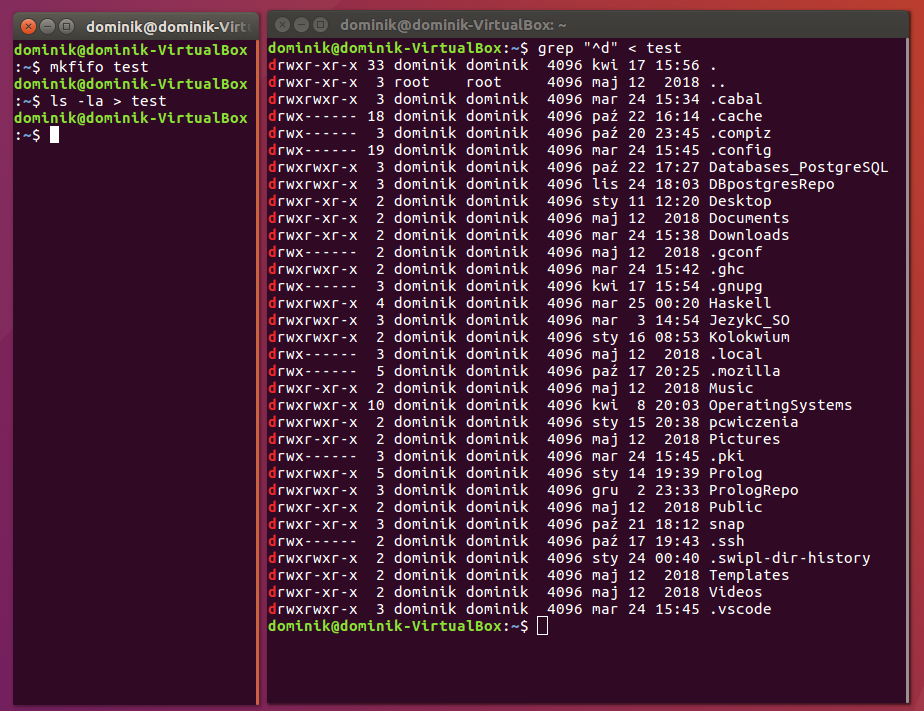
\includegraphics[scale=0.5]{zad1.png}}
%\caption{FIFO w powłoce}
%\label{fig:nazwane}
%\end{figure}
\section{Zadanie do samodzielnego wykonania}

Do wykonania wybrano zadanie \textbf{problem orangutanów}.
\assignment{ 
}{Nad głębokim kanionem, gdzieś w Ameryce Południowej, rozpięta jest lina. Używają jej orangutany by przekroczyć kanion. Lina wytrzymuje ciężar pięciu małp a dwa orangutany nie mogą jednocześnie przechodzić po niej z przeciwnych stron kanionu. Po wejściu na linę nie można zawrócić z drogi. Każda małpa oczekująca na przejście musi kiedyś zostać obsłużona.}



\begin{lstlisting}[style=CStyle, label=some-code, caption=orangutan.c]
	
  #include "line.h"
#include <stdlib.h>

int main(int argc, char* argv[]){
  
  int shmid;
  int side = -1;
  line* struktura;
  srand(time(0));

  if((shmid = shmget(4444, sizeof(line), IPC_CREAT | 0600)) == -1 ){
    perror("Utworzenie segmentu pamieci wspoldzielonej");
    exit(EXIT_FAILURE);
  }
 
  if((struktura = (line *)shmat(shmid,NULL,0)) == -1){
    perror("Przylaczanie segmentu pamieci wspoldzielonej");
    exit(EXIT_FAILURE);
  }
printf("\n");

  while(1){   
    sleep(rand()%3);
    
    if(struktura->number_of_orangutans < 2 && ( struktura->direction == side || struktura->direction == 0)){
      struktura->number_of_orangutans++;
      struktura->direction = side;
      printf("\nOrangutan %s idzie na strone %d", argv[1], side*-1);
      sleep(3);    
      struktura->number_of_orangutans--;
      if (struktura->number_of_orangutans == 0)
	struktura->direction = 0;
      side *= -1;
      printf("\nOrangutan %s jest na stronie %d", argv[1], side);
    }
    else if( struktura->number_of_orangutans == 2)
      printf("\nOrangutan %s czeka bo nie ma miejsca na linie", argv[1]);
    else
      printf("\nOrangutan %s czeka bo inny orangutani idzie w jego strone", argv[1]);
  }
  
  

  return 0;
}
	
\end{lstlisting}




\begin{lstlisting}[style=CStyle, label=some-code, caption=line.h]
	
 #include <stdio.h>
#include <sys/types.h>
#include <sys/ipc.h>
#include <sys/shm.h>
#include <stdio.h>
#include <stdlib.h>

#define MAX_ORANGUTANS 20

typedef struct{
  int number_of_orangutans; /* 0-5 */
  int left_fifo[20];         /* if conflict, first in fifo */        
  int right_fifo[20];
  int fifo_priority;        /* if conflict -1-left first 1- right first */
  int direction;            /* -1- from left to right 1-from right to left 0-free*/
} line;
	
\end{lstlisting}


\end{document}
